% ---------------------------------------------------------------------
\Needspace{8\baselineskip}\subsection{Matériel et câblage}

Le choix des pièces part de la nomenclature du projet (The Bill of Materials), où le matériel est déjà sélectionné. Il me reste à décider comment relier toutes ces pièces à un Arduino Uno, qui n'a que six entrées analogiques et une quinzaine de broches. Je cherche une solution qui limite le nombre de fils, laisse des broches libres pour la suite, et donne une mesure précise là où elle sert à prendre une décision.

Je choisis de brancher presque tous les modules sur le même bus I2C\ix{12} de l'Arduino : deux fils partagés : SDA\ix{13} (\emph{Serial Data}), qui transporte les données dans les deux sens, et SCL\ix{14} (\emph{Serial Clock}), qui transporte l'horloge envoyée par l'Arduino, chaque module ayant sa propre adresse. Cela limite le câblage et laisse libres les autres broches.

Cette sous-partie présente d'abord les capteurs et le rôle de chacun dans les décisions, puis la commande des pompes \qty{12}{V} par une carte 8 MOSFET\ix{15}. Elle regroupe ensuite tout le câblage dans un seul tableau, et se termine par le problème de perturbation entre les sondes pH et EC et la solution retenue.

\subsubsection*{Les capteurs}

Pour chaque grandeur, je me demande si elle sert à prendre une décision ou seulement à surveiller la tour. Le pH, l'EC, le niveau et la batterie commandent directement les pompes : ce sont les mesures qui doivent être les plus précises et les plus fiables. L'air et la pression servent à l'affichage. La lumière sert aussi à décider : elle indique s'il y a assez de soleil pour relancer la pompe.

Le tableau suivant donne, pour chaque capteur, son rôle dans les décisions.

\begin{table}[H]
\centering
\small
\begin{tabularx}{\textwidth}{|l|l|l|Y|}
\hline
\textbf{Grandeur} & \textbf{Capteur} & \textbf{Liaison} & \textbf{Rôle dans les décisions} \\
\hline
pH & DFRobot SEN0161-V2 & ADS1115\ix{16}, entrée A0 & dosage du pH$-$ \\
\hline
Conductivité (EC) & sonde fabriquée en graphite ($K$ de \qtyrange{0,97}{3,04}{cm^{-1}}, à étalonner) & broches D5, D6 et entrée A0 de l'Arduino & dosage des engrais \\
\hline
Niveau d'eau & ruban eTape\ix{23} \qty{30}{cm} & ADS1115\ix{16}, entrée A2 & arrêt si le réservoir est presque vide \\
\hline
Température de l'eau & DS18B20\ix{24} étanche & broche D2 (OneWire) & correction de l'EC \\
\hline
Batterie & INA260\ix{22} & I2C\ix{12} 0x40 & coupure et reprise de la pompe \\
\hline
Température, humidité de l'air & DHT20\ix{24} (Sensor Kit) & I2C\ix{12} 0x38 & affichage \\
\hline
Pression de l'air & BMP280 (Sensor Kit) & I2C\ix{12} 0x77 & affichage \\
\hline
Lumière & capteur du Sensor Kit & entrée A3 & reprise de la pompe au soleil \\
\hline
Heure & horloge DS1307 à pile & I2C\ix{12} 0x68 & dates justes même sans Internet \\
\hline
\end{tabularx}
\caption{Les capteurs et leur rôle dans les décisions.}
\end{table}

La sonde pH donne une tension analogique. Elle est lue par le convertisseur ADS1115\ix{16} (16 bits) plutôt que par l'Arduino (10 bits) : je compare les deux pas de mesure. La sonde EC, elle, est lue directement par l'entrée A0 de l'Arduino (partie 7).

\naturecalc{théorie (formule démontrée, valeurs de fiches techniques et hypothèses ; rien de mesuré)}
\begin{demonstration}[pas de mesure de l'ADS1115\ix{16} et de l'Arduino]
\resultat{q_{\mathrm{ADS}} \approx \qty{0,19}{mV}, \quad q_{\mathrm{Uno}} \approx \qty{4,9}{mV}, \quad \frac{q_{\mathrm{Uno}}}{q_{\mathrm{ADS}}} \approx 26}
Un convertisseur à $n$ bits découpe sa plage de tension en $2^n$ valeurs. Le pas $q$ est la plus petite variation de tension qu'il distingue :
\[
q = \frac{\text{plage}}{2^{n}}
\]
Pour l'Arduino, la plage va de $\qty{0}{V}$ à $\qty{5}{V}$ avec $n = 10$ bits :
\begin{align*}
q_{\mathrm{Uno}} &= \frac{\qty{5000}{mV}}{2^{10}} = \frac{\qty{5000}{mV}}{1024}\\
q_{\mathrm{Uno}} &\approx \qty{4,88}{mV}
\end{align*}
Pour l'ADS1115\ix{16}, la plage par défaut va de $-\qty{6,144}{V}$ à $+\qty{6,144}{V}$, soit une étendue de $\qty{12,288}{V}$, avec $n = 16$ bits :
\begin{align*}
q_{\mathrm{ADS}} &= \frac{\qty{12288}{mV}}{2^{16}} = \frac{\qty{12288}{mV}}{65536}\\
q_{\mathrm{ADS}} &= \qty{0,1875}{mV} \approx \qty{0,19}{mV}
\end{align*}
Le rapport des deux pas vaut :
\begin{align*}
\frac{q_{\mathrm{Uno}}}{q_{\mathrm{ADS}}} &= \frac{\qty{4,88}{mV}}{\qty{0,1875}{mV}}\\
&\approx 26
\end{align*}
L'ADS1115\ix{16} distingue donc des variations environ 26 fois plus petites. Les premières mesures réelles montrent concrètement cet écart (partie 8.8).
\end{demonstration}

\begin{attention}
\textbf{Montage actuel : une étape provisoire.} Tout le matériel n'est pas encore câblé. Depuis la mise en service du 1er novembre, l'Arduino porte le Sensor Kit (DHT20\ix{24}, BMP280 et écran), l'horloge, et la sonde pH branchée directement sur l'entrée A1 de l'Arduino, comme dans l'ancien montage. L'ADS1115\ix{16}, la carte 8 MOSFET\ix{15}, la sonde EC, la sonde de l'eau, le ruban de niveau, l'INA260\ix{22} et le capteur de lumière restent à brancher. Le câblage ci-dessus reste la référence : le programme s'adapte en attendant, et lit le pH sur A1 tant que l'ADS1115\ix{16} ne répond pas (partie 8.7).
\end{attention}

\subsubsection*{La commande des pompes}

Au début du projet, la pompe est commandée par un seul MOSFET\ix{15} branché sur la broche D3 de l'Arduino. Avec quatre pompes, cette solution demanderait quatre montages et quatre broches. La nomenclature prévoyait une carte 8 MOSFET\ix{15} pilotée en I2C\ix{12} : je la retiens parce qu'elle regroupe les transistors et les diodes de protection, n'utilise aucune broche de plus et laisse des sorties libres, que j'utilise finalement pour alimenter les sondes.

Les pompes fonctionnent en \qty{12}{V}, alors que l'Arduino ne sort que \qty{5}{V} et quelques milliampères. Elles passent donc par une carte 8 MOSFET\ix{15} (Adafruit 6318, puce MCP23017, adresse I2C\ix{12} 0x20). Chaque sortie est un transistor qui relie le fil « $-$ » de la pompe à la masse quand on l'allume ; une diode protège le circuit quand la pompe s'arrête.

Le tableau suivant liste les sorties de la carte 8 MOSFET et ce que chacune commande.

\begin{table}[H]
\centering
\small
\begin{tabularx}{0.75\textwidth}{|c|Y|}
\hline
\textbf{Sortie} & \textbf{Branchement} \\
\hline
0 & pompe principale (circulation) \\
\hline
1 & doseuse engrais A \\
\hline
2 & doseuse engrais B \\
\hline
3 & doseuse pH$-$ \\
\hline
4 & masse de la carte de la sonde pH \\
\hline
5 & libre (prévue au départ pour la carte de la sonde EC du commerce) \\
\hline
6, 7 & libres \\
\hline
\end{tabularx}
\caption{Les sorties de la carte 8 MOSFET.}
\end{table}

\begin{attention}
Le $+$ de la carte de la sonde pH va au \qty{5}{V} de l'Arduino, jamais au $+$ de la carte MOSFET\ix{15}, qui est en \qty{12}{V}. Seule sa masse passe par la sortie 4 de la carte MOSFET\ix{15}. La sonde EC fabriquée n'est pas sur la carte MOSFET\ix{15} : elle est alimentée directement par les broches D5 et D6 de l'Arduino, qui donnent tour à tour $+5$ V et $-5$ V. Les pompes ont leur borne $+$ sur la borne V+ de la carte MOSFET\ix{15} et leur autre borne sur la sortie qui les commande.
\end{attention}

\subsubsection*{Tableau de câblage}

Je regroupe tout le câblage dans un seul tableau, pour pouvoir câbler et vérifier la tour sans relire le code. Les adresses I2C\ix{12} y figurent parce que deux modules à la même adresse se brouilleraient : je vérifie qu'aucune ne se répète.

\begin{table}[H]
\centering
\small
\begin{tabularx}{\textwidth}{|l|l|Y|}
\hline
\textbf{Élément} & \textbf{Adresse / broche} & \textbf{Branchement} \\
\hline
Carte 8 MOSFET\ix{15} & I2C\ix{12} 0x20 & Vcc \qty{5}{V} ; V$+$ au \qty{12}{V} de la batterie après le fusible \\
\hline
ADS1115\ix{16} & I2C\ix{12} 0x48 & VDD \qty{5}{V}, ADDR à la masse ; A0 pH, A1 libre (l'EC est lue directement par l'Arduino), A2 ruban \\
\hline
Ruban eTape\ix{23} & ADS1115\ix{16} A2 & \qty{5}{V} $\to$ résistance \qty{560}{\ohm} $\to$ A2 $\to$ ruban $\to$ masse \\
\hline
INA260\ix{22} & I2C\ix{12} 0x40 & VIN$+$ côté régulateur, VIN$-$ côté batterie \\
\hline
Horloge DS1307 & I2C\ix{12} 0x68 & pile en place, réglée en heure UTC \\
\hline
DHT20\ix{24}, BMP280, écran OLED & I2C\ix{12} 0x38, 0x77, 0x3C & ports I2C\ix{12} du Sensor Kit \\
\hline
DS18B20\ix{24} & broche D2 & résistance \qty{4,7}{k\ohm} entre D2 et \qty{5}{V} \\
\hline
Capteur de lumière & broche A3 & port A3 du Sensor Kit \\
\hline
Raspberry Pi & USB & câble USB de l'Arduino ; vitesse \qty{115200}{bauds} \\
\hline
\end{tabularx}
\caption{Tableau de câblage.}
\end{table}

\subsubsection*{Alternance des sondes pH et EC}

La nomenclature signale déjà que la sonde EC « interfère avec la sonde pH ». Ma première idée est de simplement ignorer les mesures de pH pendant la lecture de l'EC. En étudiant le fonctionnement de la sonde EC, je comprends que cela ne suffit pas : elle perturbe l'eau tant qu'elle est alimentée, et pas seulement quand on la lit. Je décide donc de couper réellement son alimentation, avec deux sorties libres de la carte MOSFET\ix{15}.

Pour mesurer la conductivité, la sonde EC fait passer un petit courant alternatif dans l'eau. Tant qu'elle est alimentée, ce courant perturbe la sonde pH, plongée dans la même eau : le pH lu devient faux. À l'inverse, la sonde pH ne gêne pas la sonde EC.

Il ne suffit donc pas d'ignorer le pH pendant la lecture de l'EC : il faut éteindre vraiment la sonde EC quand on lit le pH. La sonde pH est coupée par la sortie 4 de la carte MOSFET\ix{15}, et la sonde EC est alimentée par les broches D5 et D6 de l'Arduino (en entrée entre deux mesures, donc déconnectée) : elles ne sont jamais actives en même temps. Le pH est lu à chaque mesure, la sonde EC étant éteinte depuis au moins \qty{5}{s}. Ensuite, une fois par minute, on éteint le pH, on allume l'EC, on attend \qty{2}{s} que la mesure se stabilise, puis on lit l'EC (la lecture elle-même ne dure que \qty{16}{ms}). Enfin, on éteint l'EC et on rallume le pH ; entre deux lectures, on garde la dernière valeur d'EC.

Le chronogramme suivant montre l'enchaînement des lectures : les deux sondes ne sont jamais alimentées en même temps.

\begin{figure}[H]
\centering
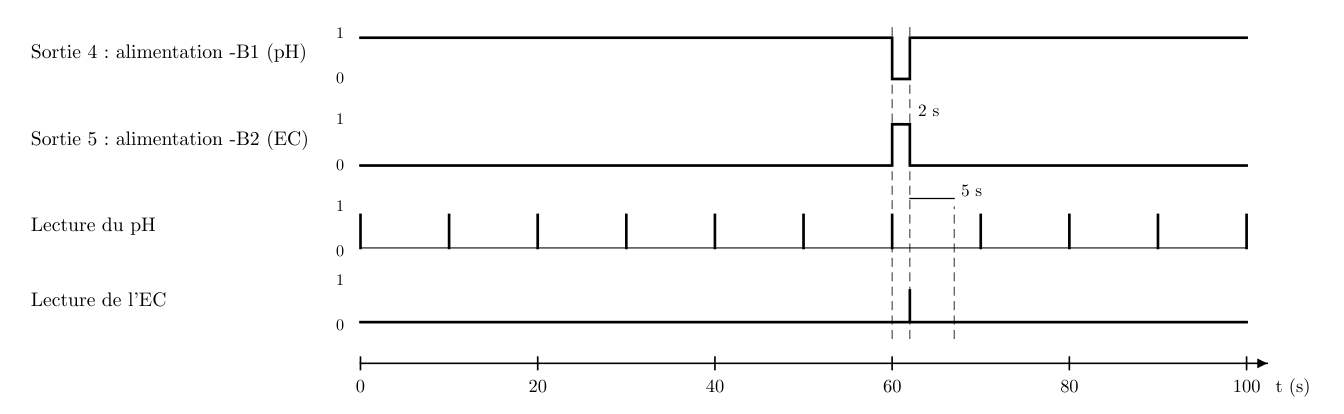
\includegraphics[width=\textwidth]{img/inf/f_chrono_sondes.png}
\caption{Chronogramme : les sondes ne sont jamais alimentées ensemble ; le pH est lu toutes les 10 s, l'EC une fois par minute, et le pH suivant attend 5 s après l'extinction de l'EC.}
\end{figure}

Le script d'essai (partie 8.9) mesure le pH sonde EC éteinte puis allumée : l'écart obtenu montrera sur la vraie tour l'intérêt de cette alternance.

% ---------------------------------------------------------------------
\Needspace{8\baselineskip}\subsection{Programme de l'Arduino}

Une fois l'organisation choisie, il faut donner à l'Arduino un programme qui lui permette d'obéir au Raspberry. Je veux un programme installé une seule fois, qu'on n'ait plus jamais besoin de modifier, mais qui garde une protection si le Raspberry tombe en panne. C'est le seul cas où j'accepte que l'Arduino prenne une décision seul. Cette sous-partie explique le choix de ConfigurableFirmata et les modules activés, puis la sécurité qui coupe les pompes quand le Raspberry ne répond plus.

\subsubsection*{ConfigurableFirmata}

Le projet utilise au départ StandardFirmata, mais cette version ne sait pas lire la sonde de température DS18B20\ix{24}, qui utilise le protocole OneWire. Plutôt que d'écrire un programme Arduino complet, je choisis ConfigurableFirmata : c'est le même protocole, enrichi de modules supplémentaires, dont le OneWire. Je n'active que les modules utiles, pour économiser la mémoire de l'Arduino Uno.

L'Arduino reçoit donc le programme \texttt{HydroTour\_Firmata}, basé sur ConfigurableFirmata. Il active seulement ce qui sert à la tour :

\begin{itemize}
\item les entrées analogiques (capteur de lumière) ;
\item le bus I2C\ix{12} (carte MOSFET\ix{15}, ADS1115\ix{16}, INA260\ix{22}, horloge, Sensor Kit) ;
\item le OneWire (sonde DS18B20\ix{24} sur D2).
\end{itemize}

À la mise en service, la compilation échoue d'abord : la version 3.3 de ConfigurableFirmata renomme une instruction (\texttt{IS\_PIN\_ANALOG} devient \texttt{FIRMATA\_IS\_PIN\_ANALOG}). Une fois corrigé, le programme occupe \qty{12870}{octets} de mémoire programme sur \qty{32256}{octets} (\qty{39,9}{\percent}, car $12870/32256 \approx 0{,}399$) et \qty{884}{octets} de mémoire vive sur \qty{2048}{octets} (\qty{43,2}{\percent}, car $884/2048 \approx 0{,}432$) : il reste de la marge pour l'Arduino Uno.

Le Raspberry s'y connecte à \qty{115200}{bauds}. Il envoie par exemple « écris 0x01 dans le registre 0x12 de la carte 0x20 » pour allumer la pompe principale, ou « lis 2 octets du registre 0x00 de l'ADS1115\ix{16} » pour obtenir une tension.

\subsubsection*{Sécurité : coupure après 30 s de silence}

En me demandant ce qui se passerait si le Raspberry plantait au milieu d'une dose, je vois le risque : la sortie resterait allumée et la doseuse viderait son flacon dans le réservoir, ou la pompe principale tournerait à sec. J'ajoute donc une surveillance dans l'Arduino. Je choisis \qty{30}{s} : c'est assez long pour qu'une mesure un peu lente ne déclenche pas de fausse coupure, et assez court pour arrêter vite une pompe oubliée.

\textbf{Limite.} Cette coupure ne remplace pas une protection locale contre la marche à sec : dans cette version, la décision d'arrêt sur niveau bas est prise par le Raspberry (partie 8.4), et si le Raspberry tombe en panne, la pompe s'arrête après \qty{30}{s} sans pour autant mesurer le niveau. Lire le niveau directement dans l'Arduino est une amélioration prévue (la première version du programme, partie 8.12, le faisait déjà). L'Arduino surveille donc les messages qu'il reçoit :

\begin{itemize}
\item le Raspberry envoie un petit message de présence toutes les \qty{5}{s}, en plus des mesures ;
\item si l'Arduino ne reçoit plus rien pendant \qty{30}{s}, il met les 8 sorties de la carte MOSFET\ix{15} à zéro, puis recommence toutes les \qty{5}{s} tant que le silence dure ;
\item dès que le Raspberry reparle, il renvoie l'état voulu des pompes à chaque mesure : tout repart normalement.
\end{itemize}

Le chronogramme suivant montre la sécurité : sans message du Raspberry pendant \qty{30}{s}, l'Arduino coupe lui-même toutes les sorties.

\begin{figure}[H]
\centering
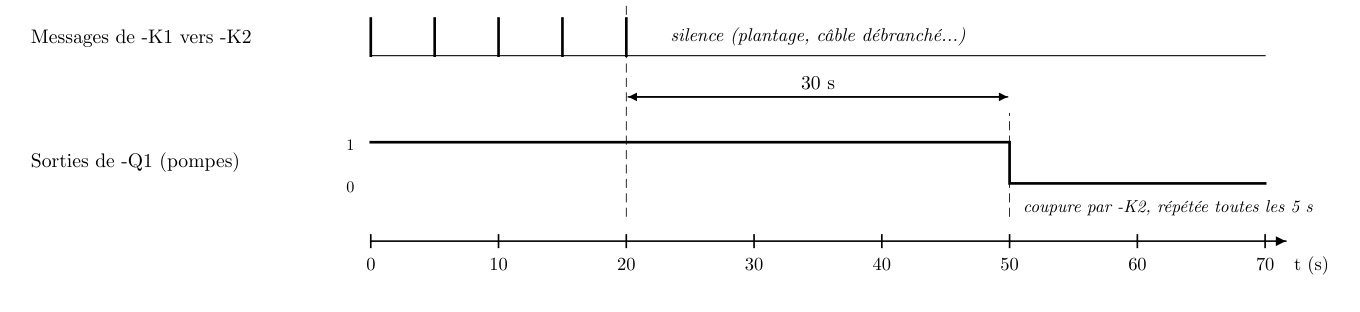
\includegraphics[width=\textwidth]{img/inf/f_chrono_secu.png}
\caption{Chronogramme de la sécurité : sans message de -K1 pendant 30 s, -K2 coupe lui-même toutes les sorties de -Q1.}
\end{figure}

